\documentclass{article}
\usepackage[utf8]{inputenc}

\usepackage{fullpage}
\usepackage{amsfonts, amsmath, pifont}
\usepackage{amsthm}
\usepackage{graphicx}
\usepackage{float}

\usepackage{tkz-euclide}
\usepackage{tikz}
\usepackage{pgfplots}
\pgfplotsset{compat=1.13}



\begin{filecontents}{q3.dat}
 n   xn
 -1  1
 0   0
 1   0  
 2   -2
 3   0
 4   3 
 5   0
 6   0
 7   -4
\end{filecontents}

\begin{document}

\begin{figure}[h!]
    \centering
        \begin{tikzpicture}[scale=1.0]
           \begin{axis}[
          axis lines=middle,
          xlabel={$t$},
          ylabel={$\boldsymbol{x(t)}$},
          xtick={-4, -3, -2, -1, ..., 4},
          ytick={-3, -2, -1, ..., 3},
          ymin=-3, ymax=3,
          xmin=-4, xmax=4,
          every axis x label/.style={at={(ticklabel* cs:1.05)}, anchor=northwest,},
          every axis y label/.style={at={(ticklabel* cs:1.05)}, anchor=south,},
          grid,
        ]
           \path[draw,line width=4pt] (-4,0) -- (-3,0) -- (-2,0) -- (-1,1) -- (1,1) -- (1,0) -- (3,0) -- (4,0);
           \end{axis}
        \end{tikzpicture}
        \caption{$t$ vs. $x(t)$.}
        \label{fig:q2}
    \end{figure}

\begin{figure} [h!]
    \centering
    \begin{tikzpicture}[scale=1.0] 
      \begin{axis}[
          axis lines=middle,
          xlabel={$n$},
          ylabel={$\boldsymbol{x[n]}$},
          xtick={ -1, 0,  ..., 7},
          ytick={-4, -3, -2, -1, ..., 4},
          ymin=-4, ymax=4,
          xmin=-1, xmax=7,
          every axis x label/.style={at={(ticklabel* cs:1.05)}, anchor=west,},
          every axis y label/.style={at={(ticklabel* cs:1.05)}, anchor=south,},
          grid,
        ]
        \addplot [ycomb, black, thick, mark=*] table [x={n}, y={xn}] {q3.dat};
      \end{axis}
    \end{tikzpicture}
    \caption{$n$ vs. $x[n]$.}
    \label{fig:q3}
\end{figure}

\begin{figure}[h!]
        \centering
        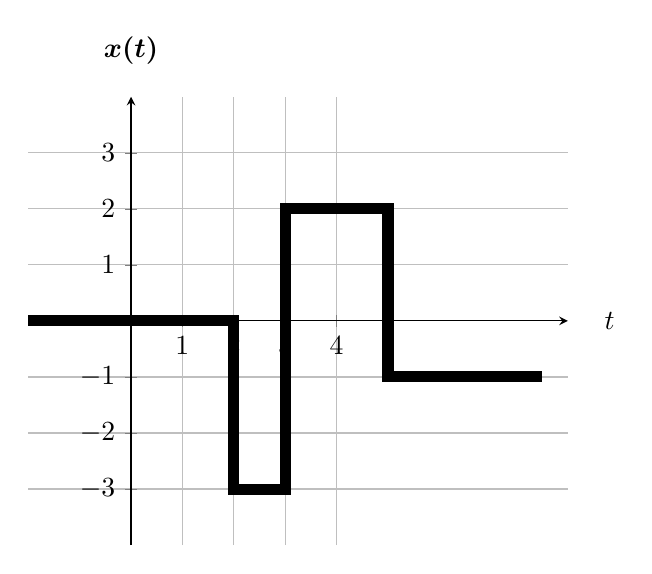
\begin{tikzpicture}[scale=1.0]
           \begin{axis}[
          axis lines=middle,
          xlabel={$t$},
          ylabel={$\boldsymbol{x(t)}$},
          xtick={0, 1, ..., 4},
          ytick={-3, -2, -1, 0, 1, 2, 3},
          ymin=-4, ymax=4,
          xmin=-2, xmax=8.5,
          every axis x label/.style={at={(ticklabel* cs:1.05)}, anchor=west,},
          every axis y label/.style={at={(ticklabel* cs:1.05)}, anchor=south,},
          grid,
        ]
           \path[draw,line width=4pt] (-2,0) -- (2,0) -- (2,-3) -- (3,-3) -- (3,2) -- (5,2) -- (5,-1) -- (8,-1);
           \end{axis}
        \end{tikzpicture}
        \caption{$t$ vs. $x(t)$.}
        \label{fig:q6}
    \end{figure}

\end{document}
